\chapter{Geometry reconstruction by lookup table}\label{ch:lookupTable}

\vspace{-1.5 em}
\begin{addmargin}[-0.5cm]{0cm}
  \minitoc
\end{addmargin}
\hrule
\vspace{1.5 em}

\noindent
We begin our attempts at reconstructing geometries by taking a very simple approach.

\section{An aside on lookup tables}
As the name would suggest, a lookup table catalogues a relationship between two sets such that anyone wishing to obtain the mapping between the sets may simply find the object of interest. Lookup tables tend to be more useful in one direction.

The idea of using a lookup table to speed up calculations is as old as mathematics itself with examples dating back to some of the earliest mathematical texts produced by ancient Egyptian scribes during the Twelfth Dynasty of Egypt (circa 1990--1800 BC) \citep[p. 1, footnote 4]{Neugebauer45}. The Egyptian Mathematical Leather Roll contains perhaps the first such complete table and tabulates 26 sums of unit fractions equaling another unit fraction. \citet{Glanville27} reports on the leather roll\footnotemark~, housed at the British Museum, and gives a photograph (figure \ref{fig:EMLR}) and schematic (figure \ref{fig:EMLRschematic}) of the table.

\footnotetext{The Egyptian Mathematical Leather Roll and the Rhine Mathematical Papyrus were both brought to the British Museum in 1864 following 1858 excavations of the tombs of Sheikh Abd el-Qurna at Thebes.}

An even more impressive lookup table is found in the extensive Rhind Mathematical Papyrus,\footnotemark~ which (seemingly) methodologically expresses the fractions $2/n$ for odd $n \in \lbrace 3, 5, \dots, 101 \rbrace$ as the sum of 2--4 unit fractions!

\footnotetext{Test.}

\begin{figure}
  \centering
  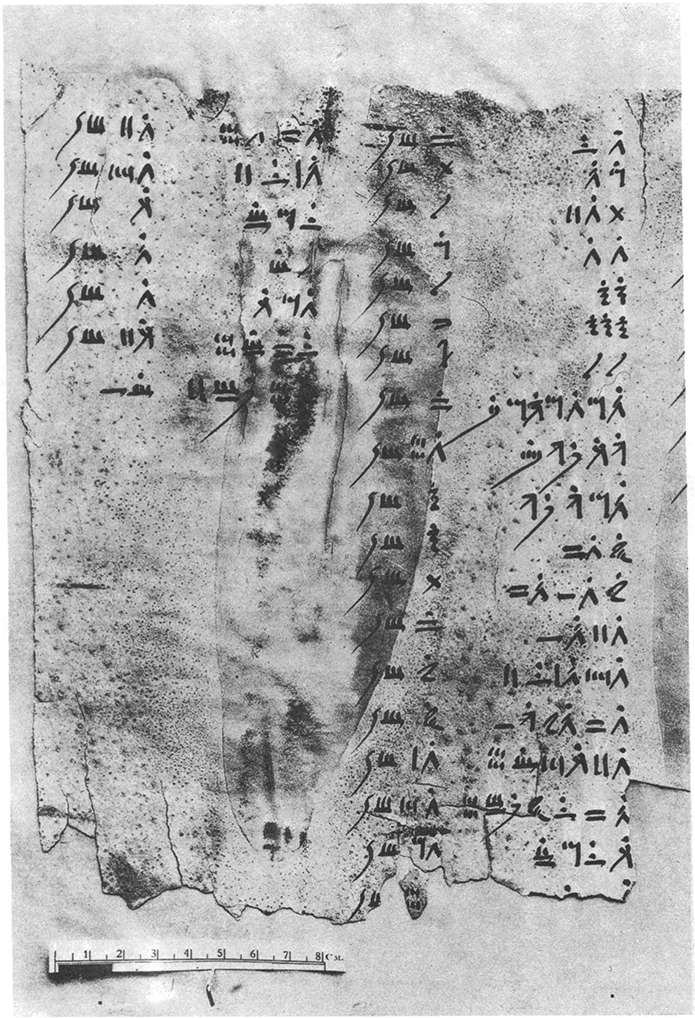
\includegraphics[width=\textwidth]{gfx/EMLR}
  \caption[Photograph of columns 3 and 4 of the Egyptian Mathematical Leather Roll.]
  {Photograph of columns 3 and 4 of the Egyptian Mathematical Leather Roll. Columns 3 and 4 are duplicates of columns 1 and 2. Figure \ref{fig:EMLRschematic} is a schematic of the table photographed here.}
  \label{fig:EMLR}
\end{figure}

\begin{figure}
  \centering
  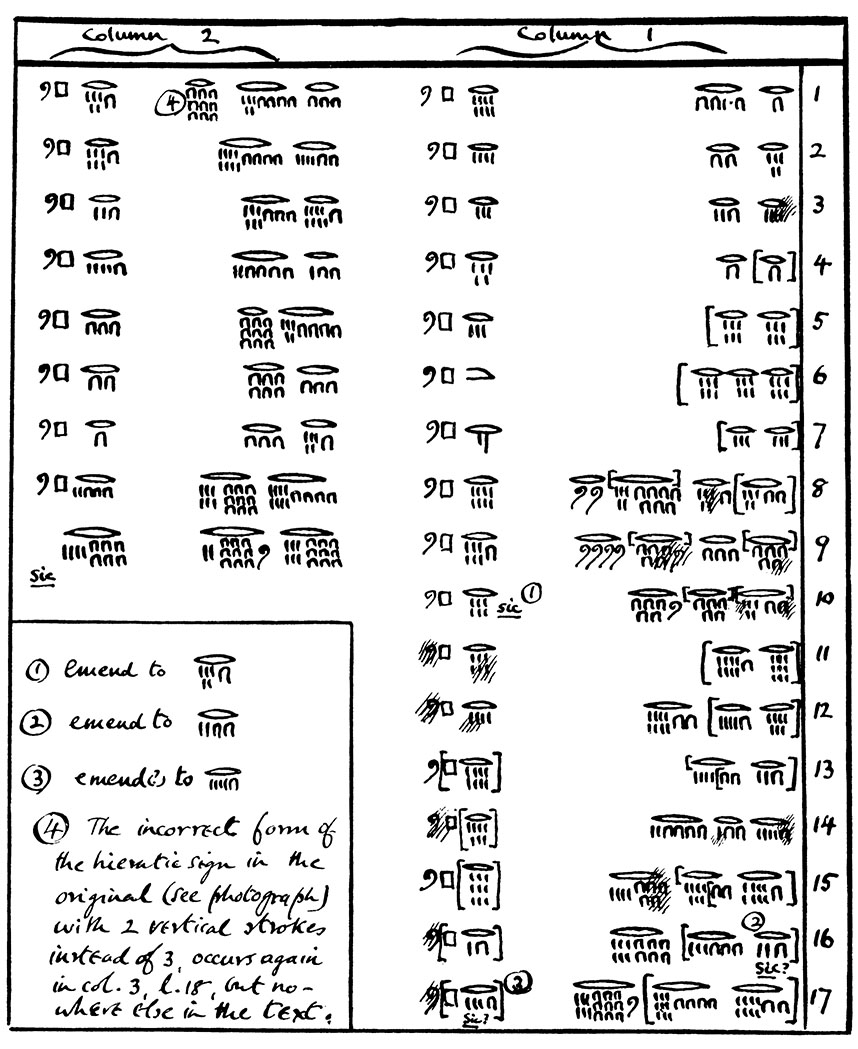
\includegraphics[width=\textwidth]{gfx/EMLRschematic}
  \caption[Schematic of columns 1 and 2 of the Egyptian Mathematical Leather Roll.]
  {Schematic of columns 1 and 2 of the Egyptian Mathematical Leather Roll. Columns 3 and 4 are duplicates of columns 1 and 2. Figure \ref{fig:EMLR} is a photograph of the table outlined here.}
  \label{fig:EMLRschematic}
\end{figure}

% Short blurby history
The most familiar lookup table may be the multiplication times table that every elementary school student is familiar where sets of two integers are mapped to their product. Lookup tables have been employed since antiquity and one of the earliest surviving examples is a 98-column multiplication table from 493 A.D. attributed to the Roman, Victorius of Aquitaine \citep{Maher01}. Before the advent of the calculator and for much of scientific history, extensive logarithm tables were used to look up their values to several decimal places and to speed up computations. The earliest such tables date back to the ancient greeks although they have since been lost, and the earliest surviving one is a sine table by the ancient Indian mathematician \={A}ryabha\d{t}a circa 499 C.E. \citep{Hayashi97}.

% Some powerful applications? Why are they used?
Of course since then lookup tables have found an enormous number of uses in computer science. Arrays are ubiquitous objects in procedural programming languages and so is the more general dictionary object, especially in Python. Sine tables are still stored in calculators for quick trigonometric computations using the CORDIC algorithm and 3D lookup tables are used in image processing to store colormaps. In each case the speed offered by a lookup table once it has been generated is the main reason for their use.

% Implementation (+ extra convergence cube)
\section{Implementation to reconstruct triatomic molecules}
\index{Lookup table}
\index{Geometry reconstruction!Lookup table}
In this approach, many Coulomb explosions are simulated (see secton \ref{sec:simulating}) using a wide variety of molecular structures as the initial condition, and the resulting momentum vectors from each simulation are stored. Thus you have a mapping from molecular structures to momentum vectors. To determine the structure belonging to a certain set of observed momentum vectors, you simply read the table in reverse. This approach is simple to implement, very quick by design, and front-loads the computation which may be desirable for large data sets. However, of course, it has an exponential time and space complexity $\mathcal{O}(e^{3N-6})$ where $N$ is the number of atoms.

\subsection{Using simulations to test accuracy}
\subsection{Computational complexity}

\section{Geometry reconstructions done by lookup table}
\subsection{A symmetric triatomic molecule: carbon dioxide}
\subsection{An asymmetric triatomic molecule: carbonyl sulfide}

\section{Conclusions and lessons learnt}
\subsection{Precision is computationally expensive}
\subsection{Difficulty in scaling to larger molecules}
\subsection{Degenerate molecular structures}

\section{Future usefulness}

% Another warning box that zooming in doesn't actually help much. If you're
% near a local minimum, you'll just zoom into that. A first go usually gives you ~ 2 sig figs of precision, anything more doesn't mean much as our momentum uncertainty is pretty high.
% Warning awesomebox that the MATLAB code has not been vectorized.